\cleardoublepage
\chapter{Impurity levels of point defects\label{ch:defects}}
In this chapter, we present the preliminary study of defect levels in semiconductors with Koopmans spectral functionals. After a brief motivation section, we discuss the two schemes used to compute the energy of the defect levels appearing within the band gap of the pristine material. Finally, we present the first results obtained for the neutral (EL2), and positively charged defect levels in gallium arsenide when one of the gallium atoms is replaced by an arsenic (As-antisite). This section represents a work in progress, and is part of the future developments following this thesis' work.

\clearpage
\section{Motivation\label{sec:motivation-defects}}
Many properties of materials are strongly influenced by the presence of impurities and point defects. Electrical and optical properties of semiconductors can be either quenched or stimulated as a consequence of the presence of defects. In extrinsic semiconductors, the hole and electron conductivities can be finely controlled by tuning the concentration of $p$-type impurity atoms -- also called acceptors, as they trap an electron and free a hole close to the top of the valence band -- and $n$-type impurity atoms -- also called donors, as they release an electron at the bottom of the conduction band. On the other hand, the presence of defect centers can also have a reversed effect and trap charge carriers in localized states, as for gold impurities in silicon \cite{corsetti_negative-u_2014}, thereby decreasing the conductivity of the material. More recently, the properties of impurity centers have been considered also in the context of quantum information, since they can represent optimal systems for quantum communication: the renowned nitrogen-vacancy (NV) center in diamond is one of them \cite{maze_properties_2011}, as it provides a very coherent optical transition that can be exploited to create an entangled state (a qubit of information). It is apparent, that many modern electronic and optoelectronic devices, are somehow affected by the presence of defects -- negatively, or positively. Understanding and being able to properly simulate such effects, is then an extremely relevant topic in computational materials science.

To test the performances of Koopmans functionals for the prediction of the position of impurity levels in semiconductors, we considered the EL2 defect in gallium arsenide. The EL2 defect has been for many years a pivotal research topic due to its influence on the electrical and optical properties of GaAs, and for its appearance during the growth process of melt GaAs, despite the total absence of any doping elements. It was observed experimentally that the EL2 concentration increases with the stoichiometry ratio of the elemental species As/Ga \cite{kaminska_el2_1987}, which hinted at a connection with arsenic. Whether the EL2 defect is associated with a substitutional As-antisite -- taking the place of a Ga-vacancy -- or with a complex of As-antisite with As-interstitials, was object of debate for a while; today, the interpretation of the simple As-antisite ($\asga$) impurity is commonly accepted. The EL2 defect level is then given by the presence of a neutral As-antisite and lies 0.75~\mev below the bottom of the conduction band \cite{kaminska_el2_1987,dabrowski_isolated_1989,komsa_assessing_2011}. The positively charged state ($\rm As_{Ga}^+$) lies instead 0.54~\mev above the top of the valence band. Given the simple nature of this defect -- the neutral As-antisite defect state is a fully symmetric ($A_1$) singlet -- and the excellent description of the band structure of GaAs from Koopmans functionals (see \cref{ch:band-structures}), the $\asga$ represents a perfect test case.

\section{Theoretical schemes\label{sec:theory-defects}}
In a mean-field approach, the Schr\"{o}dinger equation of a crystalline material, whose translation symmetry is broken by the presence of some point defect (substitutional or interstitial atoms, vacancies, dislocations, etc.), reads as
%
\begin{equation}
    -\frac{1}{2} \nabla^2 \psi + \big( V + U_{\rm d } \big) \psi = E \psi ,
    \label{eq:schrodinger-eq-defects}
\end{equation}
%
where $V$ is the periodic crystal potential, and $U_{\rm d}$ is the potential due to the presence of the impurity. Depending on the spatial extension of the wave function $\psi$, two different regimes can be identified. When the wave function spreads over the lattice, the potential $U_{\rm d}$ is much smaller than the crystal potential, thus can be treated as a small perturbation; this is the case of \emph{shallow} impurity states. Instead, when $\psi$ is localized in a small region surrounding the point defect, the impurity potential becomes dominant in that region and is the crystal potential that can be treated perturbatively; this is the case of \emph{deep} -- tightly bound -- defect states. The energy levels arising within the material's band gap, upon the formation of a shallow defect state, are usually located very close to the band edges, whereas the levels associated to deep states are much more bound and sit around mid-gap.

\begin{figure}
    \centering
    \subfloat[]{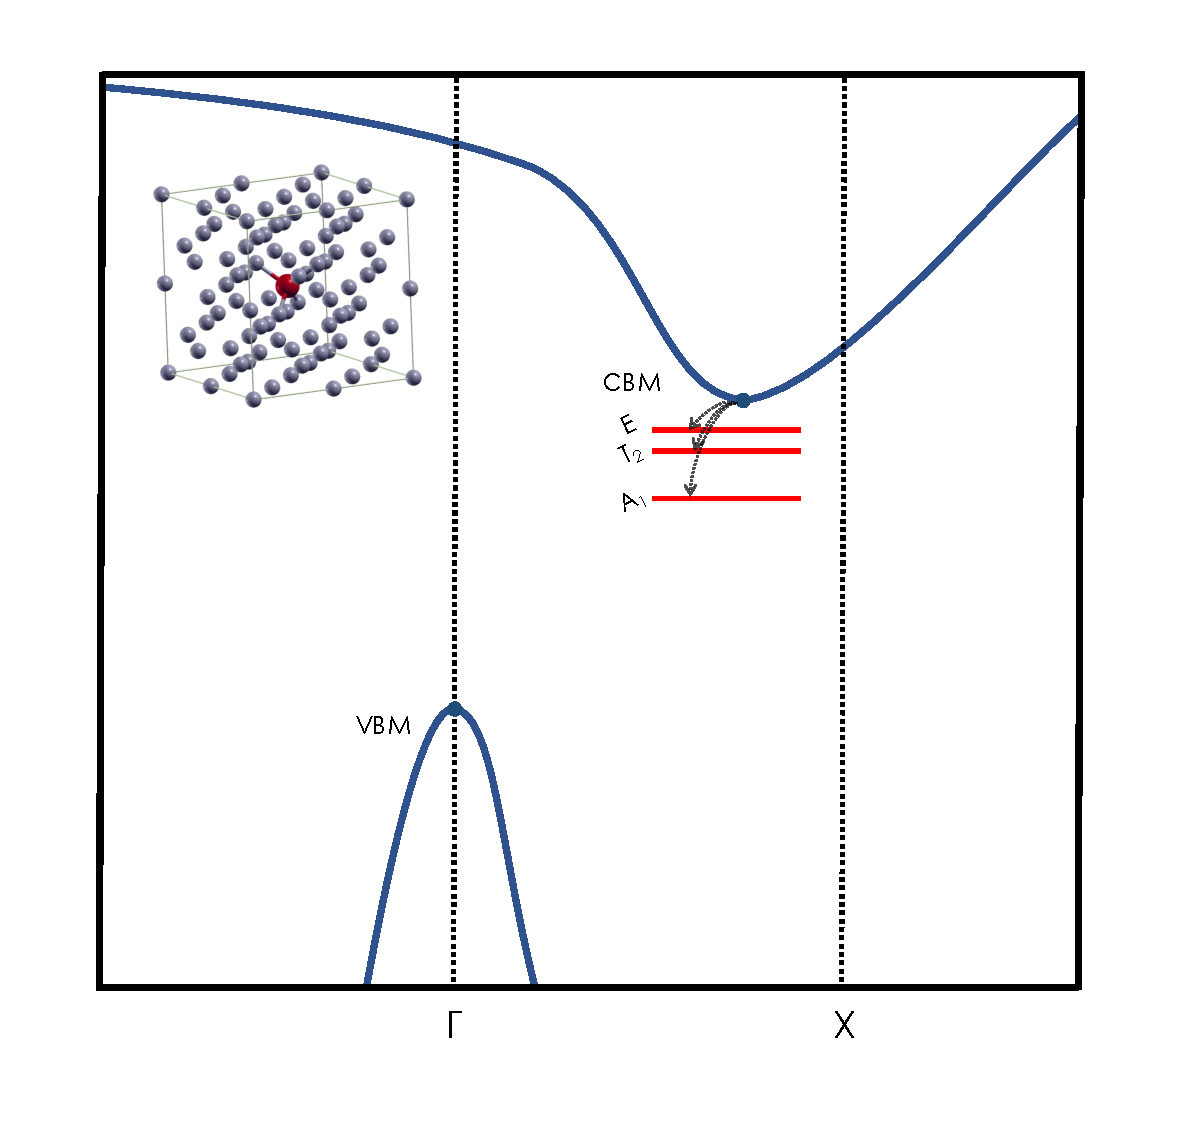
\includegraphics[width=.5\linewidth]{as-si-levels.pdf}}
    \subfloat[]{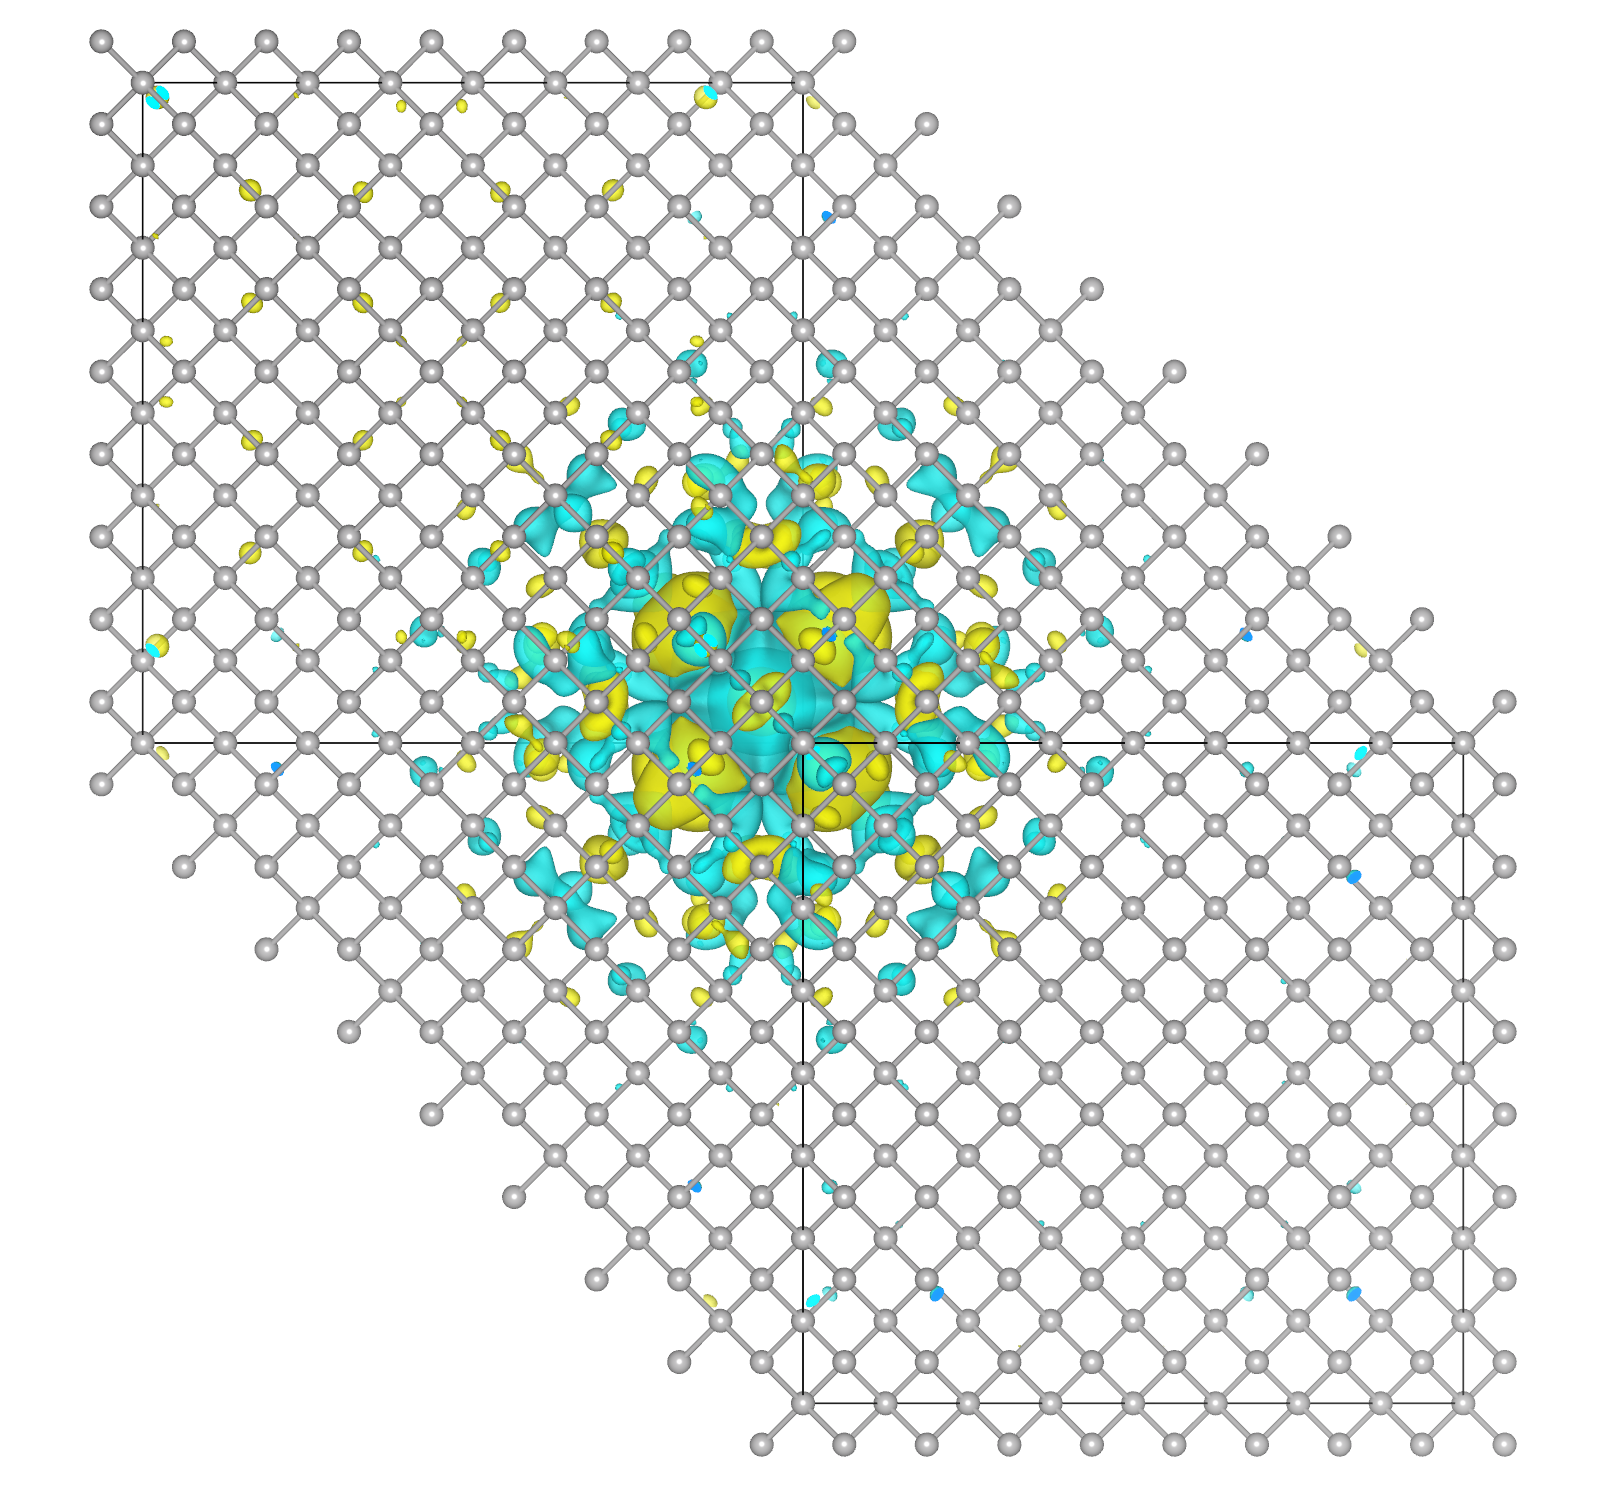
\includegraphics[width=.5\linewidth]{defect_wfc_888.png}}
    \caption[Impurity states in As-doped silicon]{Impurity states emerging in As-doped silicon. On the left, we show the three shallow energy levels forming within the band gap: a singlet ($A_1$) at 53.8~\mev below the conduction band minimum, a triplet ($T_2$) at 32.7~\mev, and a doublet ($E$) at 31.3~\mev. On the right, we show an isosurface of the orbital density of the $A_1$ defect state in a supercell containing 1024 atoms.}
    \label{fig:as-si-defect}
\end{figure}

For shallow impurities ($U_{\rm d} \ll V$), the zeroth-order Hamiltonian is that of the pristine material, therefore it is natural to represent the electronic states with Bloch functions. Historically, this type of impurities have been studied by means of the effective-mass equation, and in the Kohn-Luttinger formulation \cite{kohn_theory_1955} -- where $U_{\rm d}$ is modeled via a dielectrically screened Coulomb potential -- the predictions of the shallow donor states of silicon are in good agreement with the experiment. One of the issues with the effective-mass equation, is that it totally misses the level splitting due to the breaking of the point symmetry of the unit cell (caused by the presence of the impurity). If we consider for instance As-doped Si, the symmetry passes from $O_h$ to the smaller group $T_d$, and the six-fold degenerate conduction band minimum (CBM) splits into three groups of levels (as showed in \cref{fig:as-si-defect}). First-principles methods usually embody all the symmetries of the system, and indeed the spectrum obtained, e.g., at the DFT level, predicts the correct splitting of the energy levels. Problem is that the size of the supercell required to contain the density of a shallow defect state, can rapidly become unfeasible -- in As-doped Si it was showed that DFT results converge only for about $10^4$-atom supercells \cite{yamamoto_first-principles_2009}. For such systems, DFT represents the only possible first-principles approach, however, the intrinsic incapability of describing the electronic energies via the KS eigenvalues, demands for higher-level methods. Besides, it is worth to mention that schemes that include \emph{a posteriori} corrections of the KS eigenvalues, showed a remarkable accuracy in the prediction of the shallow donor states of silicon \cite{yamamoto_first-principles_2009,smith_ab_2017}.

Deep defect states are instead more easy to tackle from a computational point of view. The dominant character of the impurity potential ($U_{\rm d} \gg V$) in the region of the defect center, favors the localization of the wave function. The supercells used to model this type of defects contain an order of $10^2$ atoms, which makes calculations with advanced electronic-structure methods more feasible. In the following we report two possible approaches to the problem, used mainly in the context of hybrid functionals and Green's function methods, and see how those can be employed in the context of Koopmans functionals.

\subsection{The formation energy approach\label{sec:formation-energy-approach}}
The formation energy of a defect within a solid, is defined as the work required to pass from the pristine material to the system containing the impurity \cite{van_de_walle_first-principles_2004}. For a defect in the charge state $q$, the formation energy reads as
%
\begin{equation}
    E^f_{\rm d}(q) = E^{\rm tot}_{\rm d}(q) - E^{\rm tot}_{\rm bulk} - \sum_i n_i \mu_i + q \left( \varepsilon_{\rm F} + \varepsilon_{\rm v} + \Delta V \right) ,
    \label{eq:formation-energy}
\end{equation}
%
where $E^{\rm tot}_{\rm d}(q)$ and $E^{\rm tot}_{\rm bulk}$ are the total energies of the system with the defect and of the pristine material; $n_i$ is the number of atoms of species $i$ added to, or removed from the pristine system; $\varepsilon_{\rm F}$, $\varepsilon_{\rm v}$ and $\Delta V$ are the Fermi energy, the top of the valence band, and the potential alignment between the pristine material and that containing the defect. The presence of $\varepsilon_{\rm v}$ is due to the convention of referring the Fermi energy with respect to the top of the valence band.

At the DFT level, the binding energy of a defect state is defined as the transition energy between two different charge states. In this picture, the Fermi energy represents the energy of the electronic reservoir, that can be tuned in order to identify the most stable configuration. As showed in \cref{fig:formation-energy}, the transition between two different charge states $q$ and $q'$ occurs when two formation energy curves cross each other: the intersection point provides the energy of the impurity state, $\varepsilon(q/q')$. The expression for $\varepsilon(q/q')$ is then given by the solution of the equation for $\varepsilon_{\rm F}$ fulfilling the condition $E^{\rm tot}_{\rm d}(q) = E^{\rm tot}_{\rm d}(q')$ \cite{chen_first-principles_2015}:
%
\begin{equation}
    \varepsilon(q/q') = \frac{E^{\rm tot}_{\rm d}(q) - E^{\rm tot}_{\rm d}(q')}{q' - q} -\varepsilon_{\rm v} - \Delta V .
    \label{eq:energy-defect-level}
\end{equation}

In order to solve \cref{eq:energy-defect-level}, we need to: (i) compute the total energies of the system with the impurity in the two charge states $q$ and $q'$, (ii) calculate the band structure of the pristine material (or at least determine the energy of the top of the valence band), and (iii) align the energy reference of the system with and without defect. The potential alignment can be performed by comparing the planar averages of the electrostatic potential in a region far from the defect; alternatively, one can compute other quantities that are supposed to match in the bulk region, such as the expectation value of the crystal Hamiltonian over a Wannier function (again, localized in a region which, ideally, is unaffected by the presence of the impurity). We highlight that when computing total energies in charged systems, finite-size effects must be properly accounted for (see \cref{sec:makov-payne}).

\begin{figure}
    \centering
    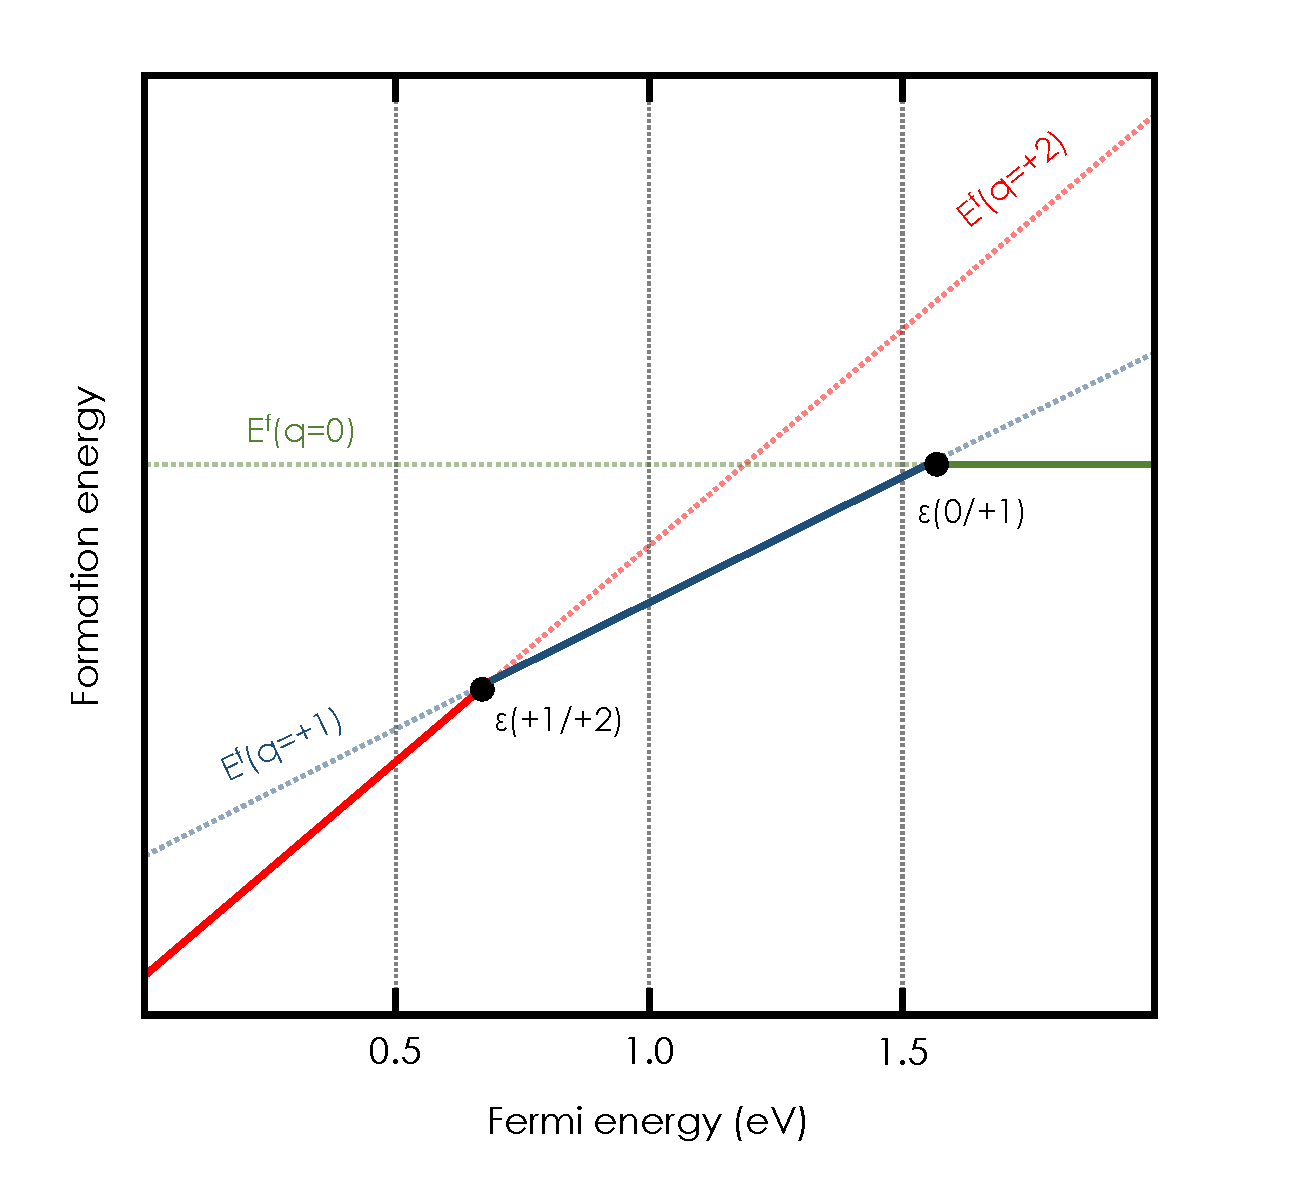
\includegraphics[width=.6\linewidth]{formation-energy.pdf}
    \caption[Charge-transition states obtained from the defect formation energy]{Defect formation energies for different charge states ($q=0$ green, $q=+1$ blue, $q=+2$ red) as a function of the Fermi energy. In this example, reproducing qualitatively the trend of $E^f_{\rm d}$ for the As-antisite in GaAs, the continuous piecewise-linear line gives the most stable configuration. Two transitions, each of them involving the loss of an electron, occur at the crossing points between two formation energy curves.}
    \label{fig:formation-energy}
\end{figure}

Any approach able to compute the quantities involved in \cref{eq:energy-defect-level} can be used, in principle, to calculate the energy of defect states. In the framework of DFT one usually resorts to local or semi-local functionals or, for more accurate predictions, to hybrid functionals. Koopmans functionals can be also used in this context. For the KI functional, whose energy at integer particle numbers equals that of the underlying DFT functional, this strategy is quite straightforward: the total energies can be computed at the DFT level, whereas the band edges can be obtained from a KI calculation. Indeed, as we saw both in theory (\cref{ch:koopmans-theory}) and in the results obtained here (\cref{ch:band-structures}) and in previous works \cite{nguyen_koopmans-compliant_2018,colonna_koopmans-compliant_2019}, Koopmans functionals provide individual corrections to the orbital energies, meaning that they predict the absolute position of the quasiparticle energies (and not just the relative shift). In this way, computing the energy of impurity levels requires KI calculations only for the pristine material. At the KIPZ level, the underlying functional is the (screened) PZ functional, which should be then used to compute total energies. However, in first approximation, one could still compute the energy differences from a standard density-functional, and apply shift of the band edges computed from a KIPZ calculation. This approach is particularly effective in systems where the defect state is localized: in these cases the delocalization error is minimized, and the total energies computed from local or semi-local functionals and from hybrid approaches -- and, presumably, from the PZ functional -- are very similar \cite{komsa_assessing_2011}.

\subsection{The quasiparticle approach\label{sec:defect-quasiparticle-approach}}
For methods whose orbital energies reproduce accurately quasiparticle excitations, the position of defect states for a charge-transition from $q$ to $q+1$ can be computed as \cite{chen_first-principles_2015}
%
\begin{equation}
    \varepsilon(q/q+1) = \left[ E(q+1,\bR_q) - E(q,\bR_q) \right] + \left[ E(q+1,\bR_{q+1}) - E(q+1,\bR_q) \right] .
    \label{eq:defect-energy-quasiparticle}
\end{equation}
%
The first term between square brackets represents the unrelaxed ionization energy ($\bR_q$ is the equilibrium geometry for the system with charge $q$), whereas the effects due to structural relaxations, following the electron or hole removal processes, are accounted for via the second term. The energy of the defect state can be evaluated from \cref{eq:defect-energy-quasiparticle} when MBPT methods, such as the \gw approximation, are employed, in combination with a DFT computation of the structural relaxation energy. We highlight that, as an alternative to MBPT, similar calculations were carried out with remarkable results using the PZ functional \cite{gudmundsdottir_calculations_2015}. In this context, also Koopmans functionals are perfectly suitable since they directly provide the charged excitations of the system. Differently from the approach based on the formation energy, here the Koopmans calculation must be performed for the system embedding the impurity, which generally is computationally more demanding. On the other hand, it possibly provides a more complete treatment of the problem, as it accounts for effects that are not considered by the approach described in the previous section -- such as the different shift of the band edges in the system with and without the defect.

\section{Results and discussions\label{sec:defects-results}}
In this section we show the preliminary results obtained by means of the two procedures described in the previous section. As mentioned earlier, the defect levels considered in this work come from the As-antisite in GaAs: in the notation introduced ealier, the neutral $\asga$ defect level (EL2) is given by $\varepsilon(+1/0)$, while the positively charged $\asga^+$ is given by $\varepsilon(+2/+1)$.

Starting from the formation energy approach, we compared the results obtained from Koopmans functionals with Komsa and Pasquarello \cite{komsa_assessing_2011}, who considered different types of hybrid functionals: HSE, PBE0, tHSE, and tPBE0, where in the last two hybrids the mixing parameters are tuned to match the experimental band gap. To focus on the electronic effects and avoid any possible discrepancies coming from the differences in the structure or in the parameters used in the calculations, we took the values for the PBE defect levels from Ref.~\cite{komsa_assessing_2011}. In that work, the total energies were computed on the HSE relaxed structure using the experimental lattice parameter, and the finite-size effects were corrected by means of the method proposed by Freysoldt \emph{et al.} \cite{freysoldt_fully_2009}. The energy of the defect states at the Koopmans level was then computed by shifting the PBE band edges of the pristine GaAs, as obtained from a Koopmans band structure calculation. The results are reported in \cref{fig:defect-level-formation-energy}. The EL2 defect level is slightly overestimated, but the accuracy is comparable to that of optimally tuned hybrid functionals. Once more, we remark that while in Ref.~\cite{komsa_assessing_2011} the total energies were computed each time at the hybrid level, the results obtained from Koopmans functionals rely simply on PBE total energies. Regarding the charged $\asga^+$ state, the results obtained from pKIPZ and KIPZ are in perfect agreement with the experiment, and also KI shows a good accuracy.

\begin{figure}
    \centering
    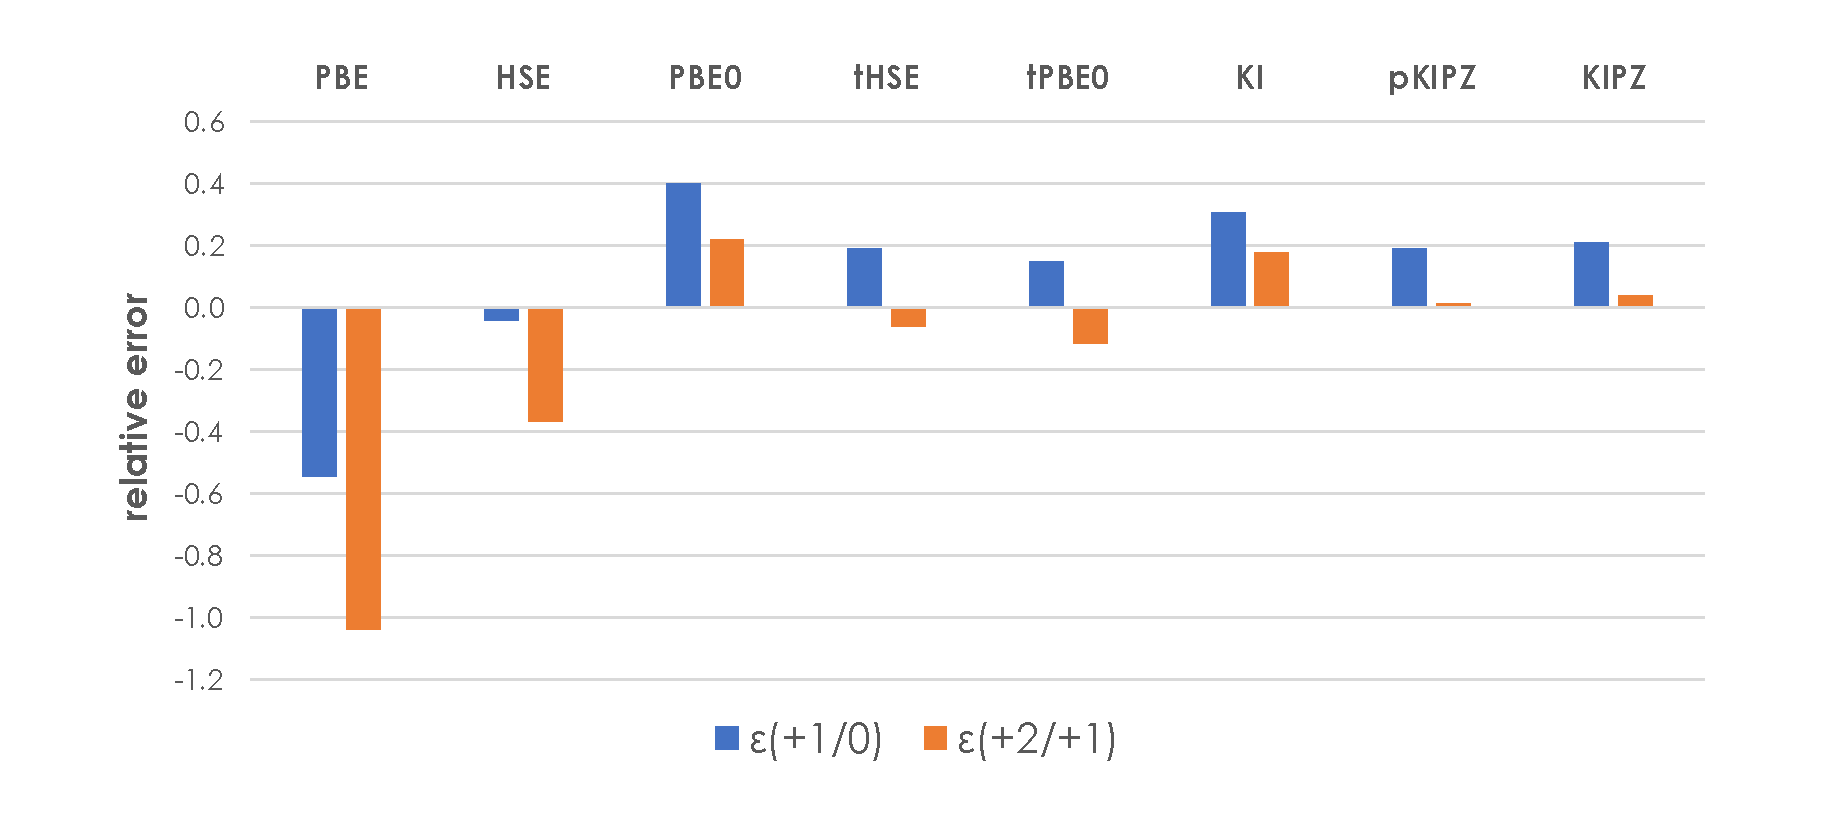
\includegraphics[width=\linewidth]{relative-error-defects.pdf}
    \vspace{5mm}
    %
    \begin{tabularx}{\linewidth}{*{1}{>{\arraybackslash}>{\hsize=2cm}X}*{9}{>{\centering\arraybackslash}X}}
        \hline
        \hline
                             &    PBE &   HSE &  PBE0 &  tHSE & tPBE0 &    KI & pKIPZ &  KIPZ &  Exp \\
        \hline
        $\varepsilon(+1/0)$  &  0.349 & 0.737 & 1.076 & 0.916 & 0.884 & 1.006 & 0.916 & 0.931 & 0.77 \\
        $\varepsilon(+2/+1)$ & -0.021 & 0.341 & 0.657 & 0.507 & 0.476 & 0.636 & 0.546 & 0.561 & 0.54 \\
        \hline
    \end{tabularx}
    %
    \vspace{5mm}
    %
    \caption[$\varepsilon(+1/0)$ and $\varepsilon(+2/+1)$ defect states of As-antisite in GaAs from hybrid and Koopmans functionals]{Comparison of the $\varepsilon(+1/0)$ and $\varepsilon(+2/+1)$ defect states (in \ev) of As-antisite in GaAs, calculated from different hybrid functionals \cite{komsa_assessing_2011} and from the three Koopmans flavors. All the values are referred to the top of the valence band and include a correction of 0.1~\ev due to spin-orbit coupling. In the bar plot above, we report the relative errors for each method.}
    \label{fig:defect-level-formation-energy}
\end{figure}

\begin{table}[b]
    \centering
    \begin{tabularx}{0.7\linewidth}{*{1}{>{\arraybackslash}>{\hsize=2cm}X}*{9}{>{\centering\arraybackslash}X}}
        \hline
        \hline
                            &   PBE &   KI & pKIPZ &   Exp \\
        \hline
        $\varepsilon(+1/0)$ &  0.05 & 0.63 &  0.59 &  0.77 \\
        \hline
    \end{tabularx}
    \caption[EL2 state from the quasiparticle approach]{Energy (in \ev) of the EL2 state of GaAs computed via the quasiparticle approach.}
    \label{tab:defect-state-quasiparticle}
\end{table}

We then considered the ``quasiparticle approach'' and performed calculations of Koopmans functionals directly on the SC containing the antisite arsenic. For the moment we report the results only for the KI and pKIPZ functionals, as the KIPZ minimization brings to a possibly nonphysical hybridization of the defect state with other variational orbitals, which requires a more detailed analysis. As for standard band structure calculations, the variational orbitals used for the two Koopmans flavors are Wannier functions; however, rather than employing MLWFs, here we used projected WFs (see \cref{sec:results-dfpt}) resulting from the simple projection of the KS Bloch states onto the selected atomic-like projectors. Moreover, the KS wave function corresponding to the defect state has not been modified when applying the Koopmans correction, in order to avoid the unwanted mixing of this state with other electronic wave functions. This is possible since, already at the PBE level, the orbital density of the defect state is sufficiently localized in space to undergo a significant Koopmans correction. The calculations were carried out only on the neutral system (access only to the EL2 state), using a $4\times 4\times 4$ SC which, as showed in \cref{fig:extension-defect-state} seems to be sufficiently large to converge the density of the defect state. The results are reported in \cref{tab:defect-state-quasiparticle}, where the energy of the impurity state corresponds to the separation between the eigenvalues corresponding to the defect state and to the top of the valence band (as for the values reported in \cref{fig:defect-level-formation-energy}, $\varepsilon_{\rm v}$ was shifted up of 0.1~\ev due to spin-orbit effects). The energy due to structural relaxations -- quantity given by the second energy difference on the right-hand side of \cref{eq:defect-energy-quasiparticle} -- was computed at the PBE level, and displayed a non-significant contribution (less than 0.01~\ev).

\begin{figure}
    \centering
    \subfloat[]{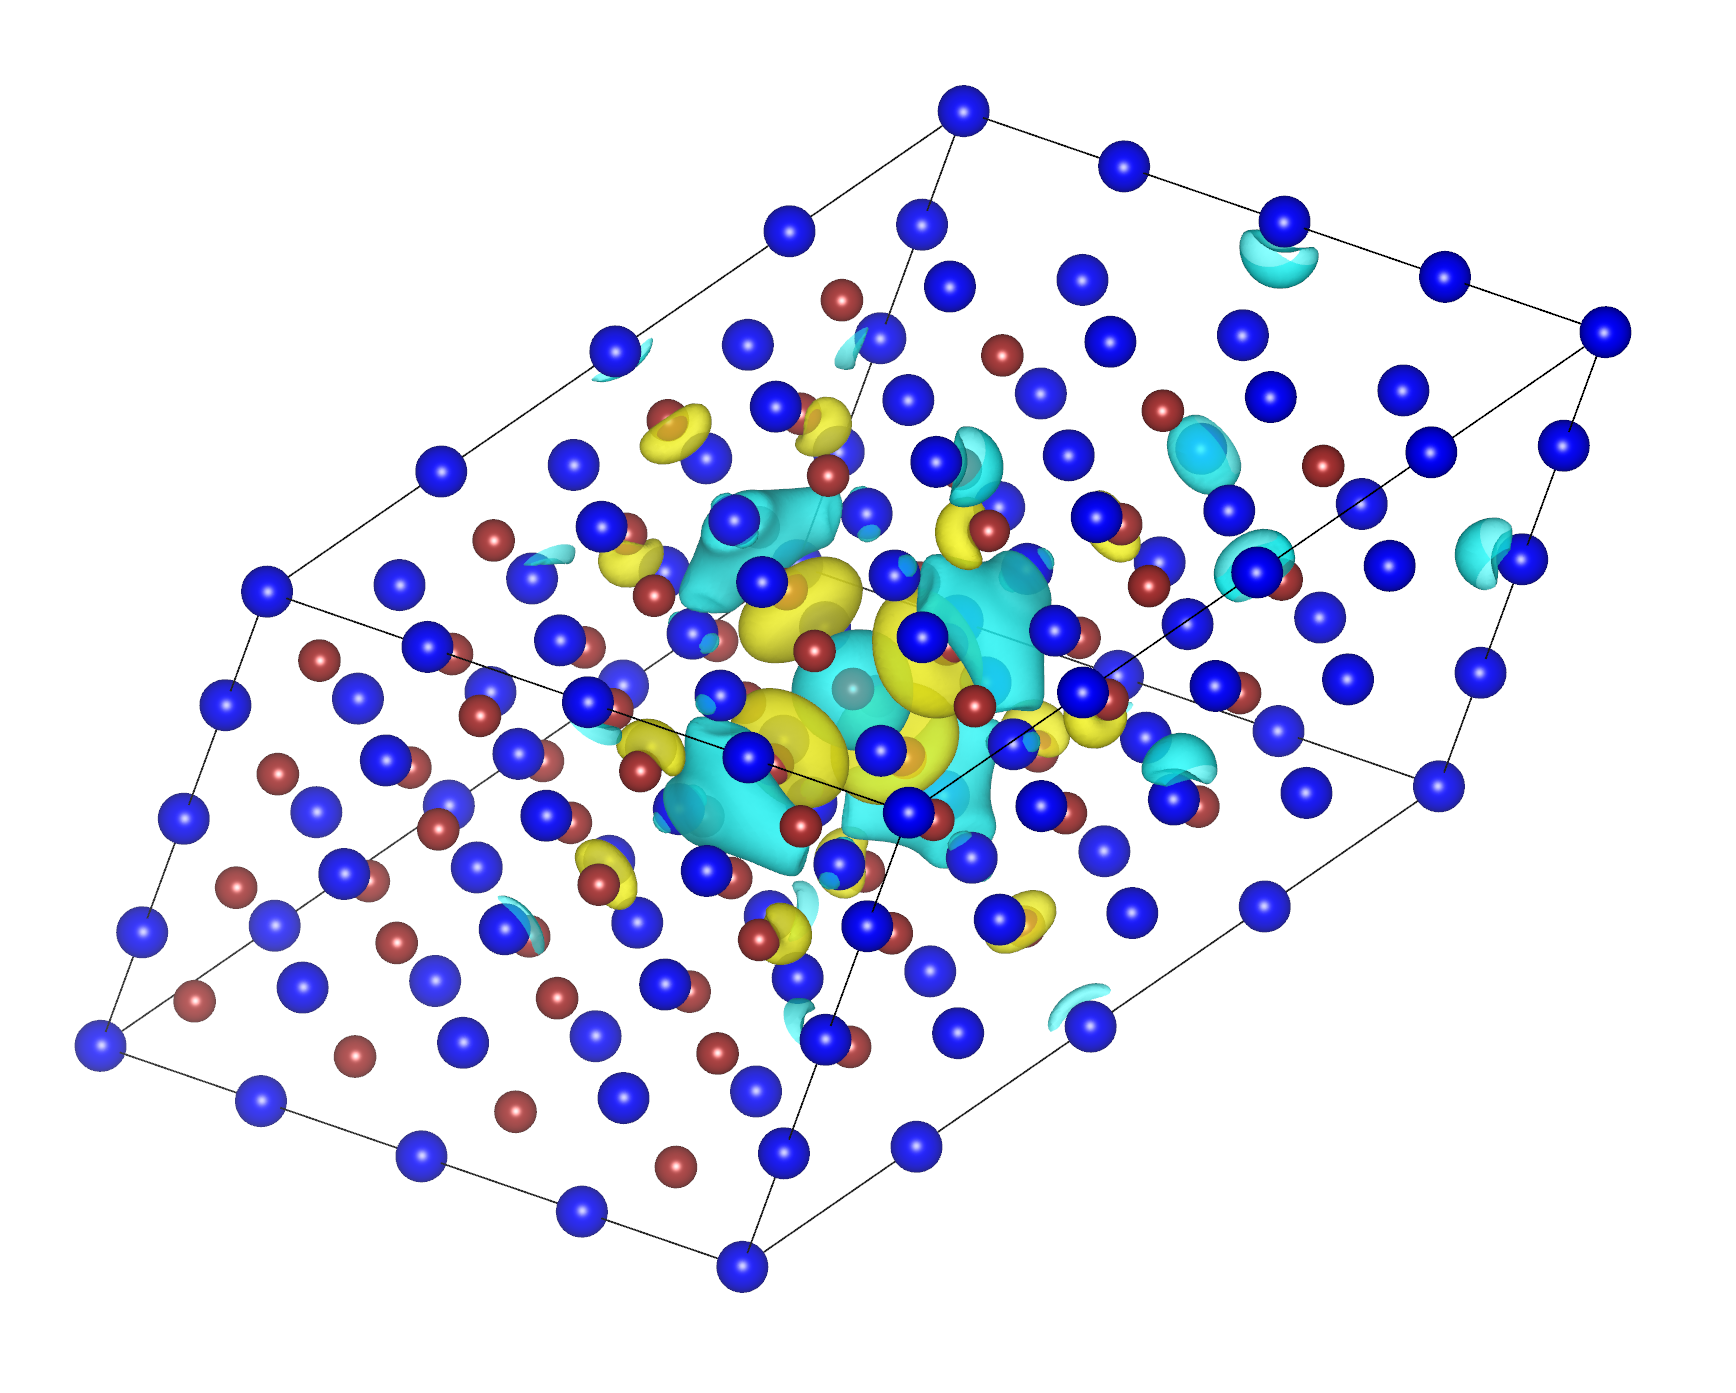
\includegraphics[width=.4\linewidth]{as-gaas-defect.png}} \qquad
    \subfloat[]{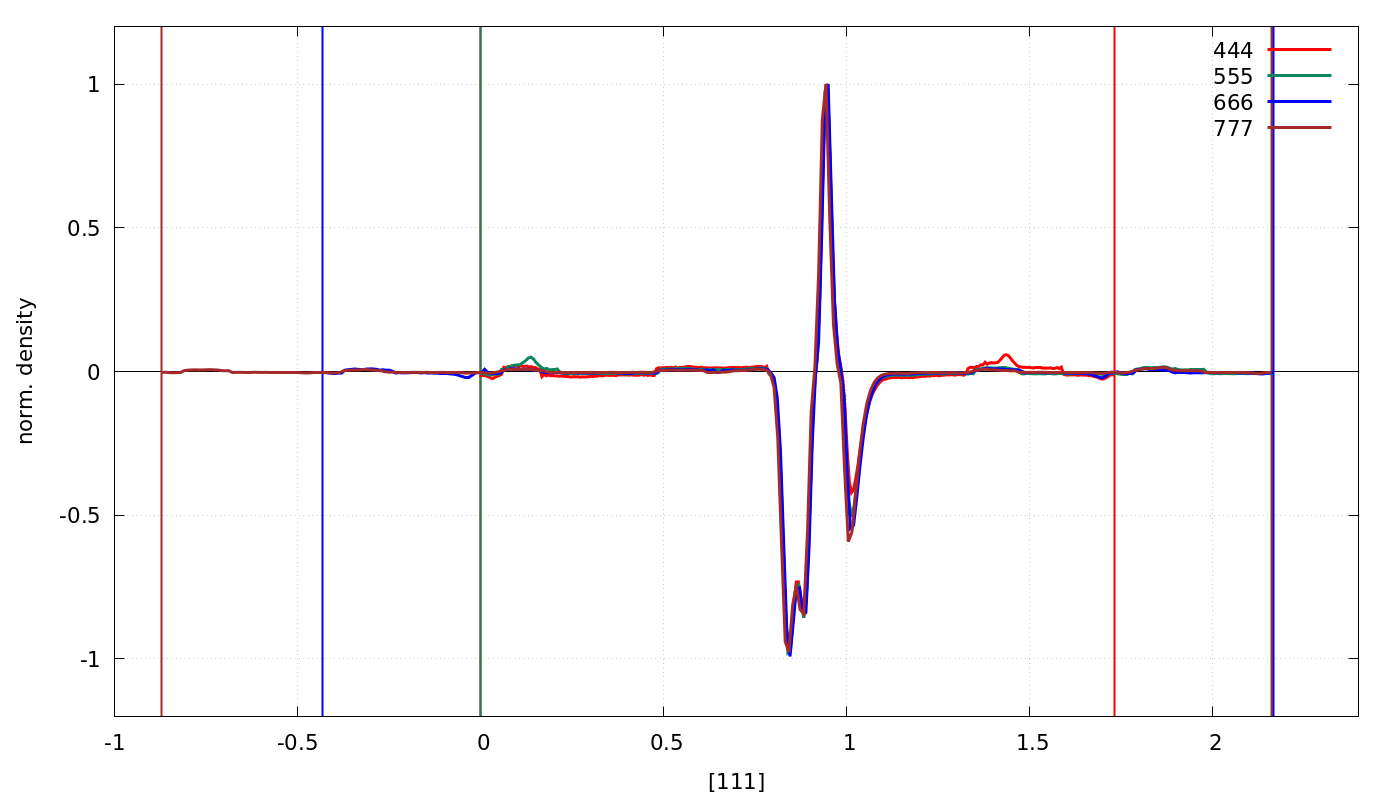
\includegraphics[width=.5\linewidth]{as-gaas-defect-extension.png}}
    \caption[Density distribution of the EL2 state]{Density distribution of the EL2 state: in (a) we show a particular isosurface which highlights the expected tetrahedral symmetry of the wave function, and in (b) we show the profile, along the $[111]$-direction, of the density for SCs of different sizes.}
    \label{fig:extension-defect-state}
\end{figure}

For the EL2 state, the results obtained with Koopmans functionals seem to agree much more with the experiment. Especially for the KI functional, this is somehow unexpected and in the following we will try to explain why. As discussed in \cref{ch:koopmans-theory}, the KI corrective term, $\Pi_i^{\rm KI}$, replaces the mistaken derivative of the underlying functional (PBE in this case) with a linear term given by the constrained $\Delta$SCF energy corresponding to the emptying (or filling) of the $i$-th orbital [see, e.g., \cref{eq:pi-term-general}]. In first approximation, the Koopmans eigenvalues correspond then to a $\Delta$SCF energy computed at the level of the underlying functional, which is exactly the way we calculate the position of defect levels from the formation energy approach [see \cref{eq:energy-defect-level}]. According to this line of reasoning, the two approaches should give similar results. The differences observed might be due to several factors. One possibility is that the off-diagonal elements of the Koopmans Hamiltonian -- normally less important, given the strong localized character of the variational orbitals -- give a significant contribution, and slightly modify the $\Delta$SCF value. We believe that in this specific case, where the wave function of the defect state is unchanged when the KI correction is applied, the KI Hamiltonian is almost block-diagonal, and the off-diagonal elements mixing the defect state with other orbitals are all zero. The KI eigenvalue corresponding to the defect state is \emph{really} equal to the PBE $\Delta$SCF energy. Nevertheless, in general, there might be an effect due to the off-diagonal matrix elements, especially for the pKIPZ and KIPZ functionals, and the comparison with the $\Delta$SCF might be less straightforward. Another source of discrepancy between the two approaches, is given by the fact that the Koopmans correction shifts differently the band edges of the system with defect, with respect to the pristine material. Already at the PBE level, the separation between the band edges, i.e. the fundamental gap, is slightly modified (of about 10\%) when the impurity is inserted. Upon the application of the Koopmans correction, the shift of the band edges is about 0.1~\ev smaller than in the pristine system, which is not accounted for in \cref{eq:energy-defect-level}, and partially justifies the differences in the two results.

\begin{figure}
    \centering
    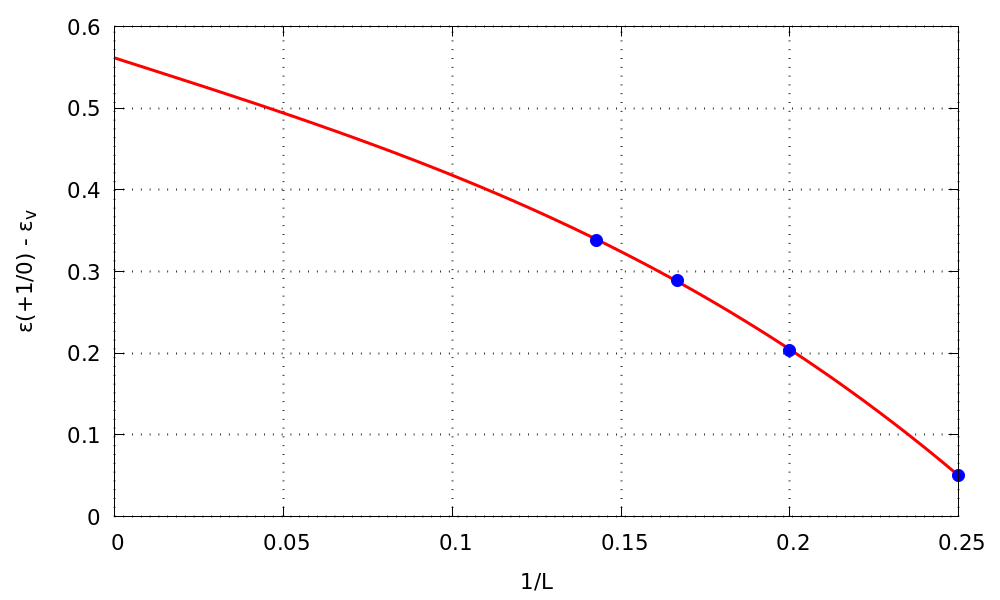
\includegraphics[width=.58\linewidth]{defect-level-vs-scell.png}
    \caption[Convergence study of the defect KS eigenvalue]{PBE HO eigenvalue corresponding to the EL2 defect state, for SCs of different size. The fit was performed using the three-parameter function $f(L) = a + b/L + c/L^3$.}
    \label{fig:convergence-ks-eig-defect}
\end{figure}

Ultimately, there might be a convergence issue. As showed in \cref{fig:convergence-ks-eig-defect} the convergence of the KS eigenvalue corresponding to the impurity state, is extremely slow with respect to the size of the SC. This aspect is not yet understood as the convergence studies of the average electrostatic potential, as well as the profile of the density of the defect state showed in \cref{fig:extension-defect-state}, displayed converged results already on the $4\times 4 \times 4$ SC. On the other hand, if the $\Delta$SCF interpretation of the Koopmans eigenvalues were to be correct, this convergence issue would probably be avoided since, for localized defects, total energy differences converge much faster \cite{komsa_assessing_2011}. Yet, a more detailed analysis of the behavior of Koopmans functionals in defect calculations is required, in order to fully understand the differences between the formation energy and the quasiparticle approach.

To summarize, the formation energy approach allows to compute the energies of defect levels in a very efficient way, which involves DFT calculations of total energies for the system containing the impurity, and Koopmans band structure calculations for the pristine material. In the case the As-antisite impurity in GaAs, the results displayed an accuracy comparable to that of hybrid functionals for the EL2 state, and an almost perfect agreement with the experiment for the positively charged state. The quasiparticle approach produced results that are unexpectedly different from those obtained from the formation energy, but in much better agreement with the experiment. The method is more complex in this case, as it requires performing calculations with Koopmans functionals on the system with the defect, but it is considered to be more rigorous, since it accounts for possible differences in the Koopmans correction of the band edges. Besides, different components might play a role in this case, and further studies are needed.

%In \cref{fig:avg-pot} we report the convergence study for the average electrostatic potential, computed on SCs of different sizes all containing the As-antisite: for all the SCs considered, the electrostatic potential in the ``bulk'' region was the same, indicating the quick convergence of the total density for this system. From the comparison with the average electrostatic potential of the pristine material, we obtained the value of 20~\mev for the potential alignment which does not affect significantly the results\footnote{
%Although the potential alignment was already included in the value taken from Ref.~\cite{komsa_assessing_2011}, a 
%}

%\begin{figure}
%    \centering
%    \sbox{\measurebox}{
%        \begin{minipage}{.5\linewidth}
%            \subfloat{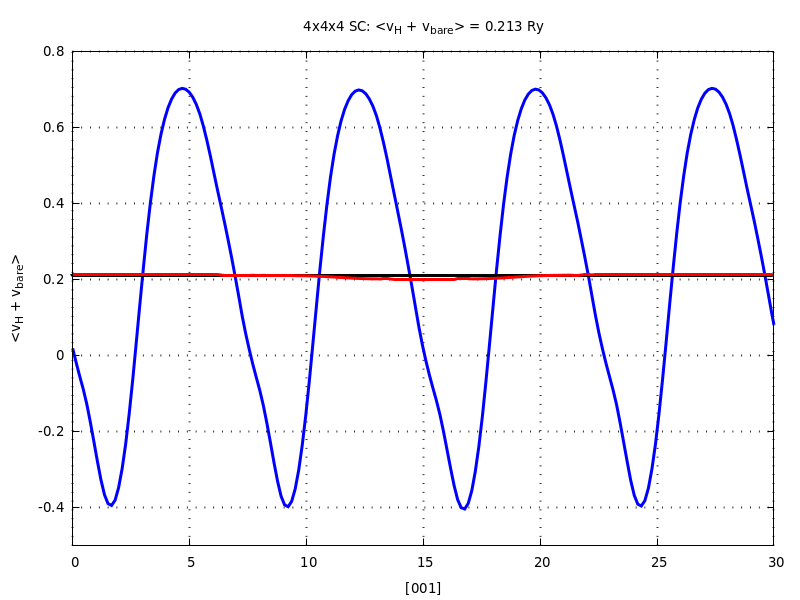
\includegraphics[width=.5\linewidth]{avg_pot_444.png}}
%            \subfloat{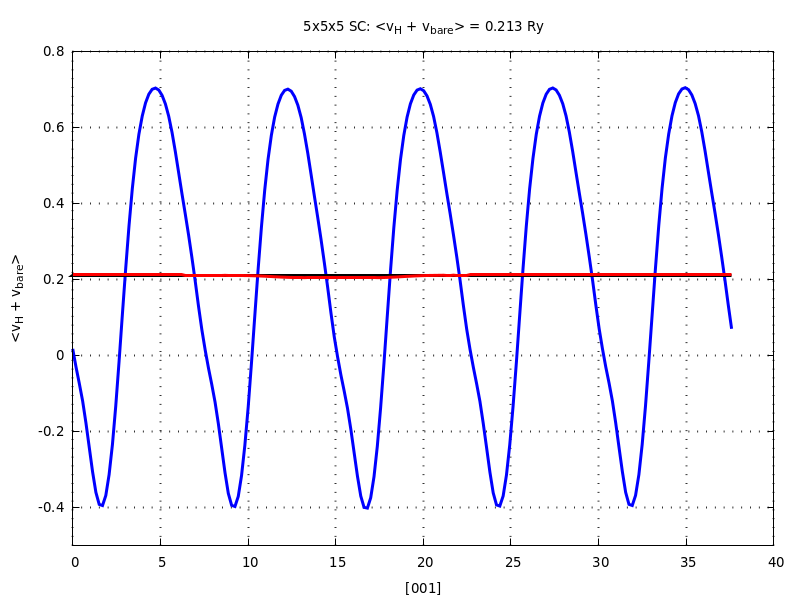
\includegraphics[width=.5\linewidth]{avg_pot_555.png}} \\
%            \subfloat{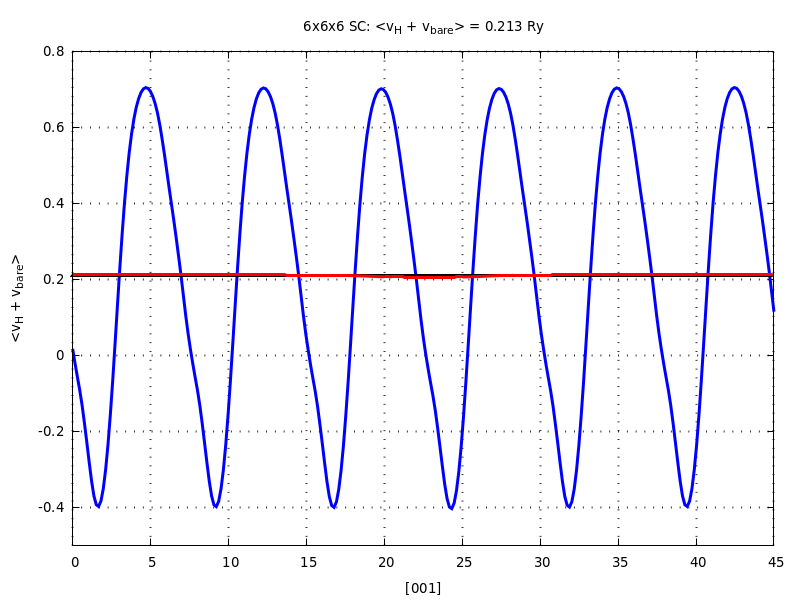
\includegraphics[width=.5\linewidth]{avg_pot_666.png}}
%            \subfloat{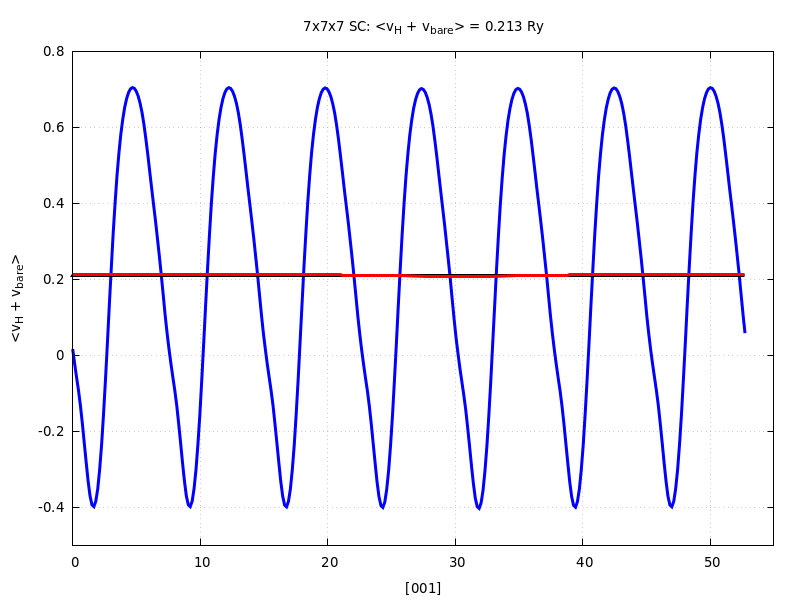
\includegraphics[width=.5\linewidth]{avg_pot_777.png}} \\
%        \end{minipage}
%    }
%    \usebox{\measurebox}
%    \begin{minipage}{.48\linewidth}
%        \vspace{5mm}
%        \subfloat{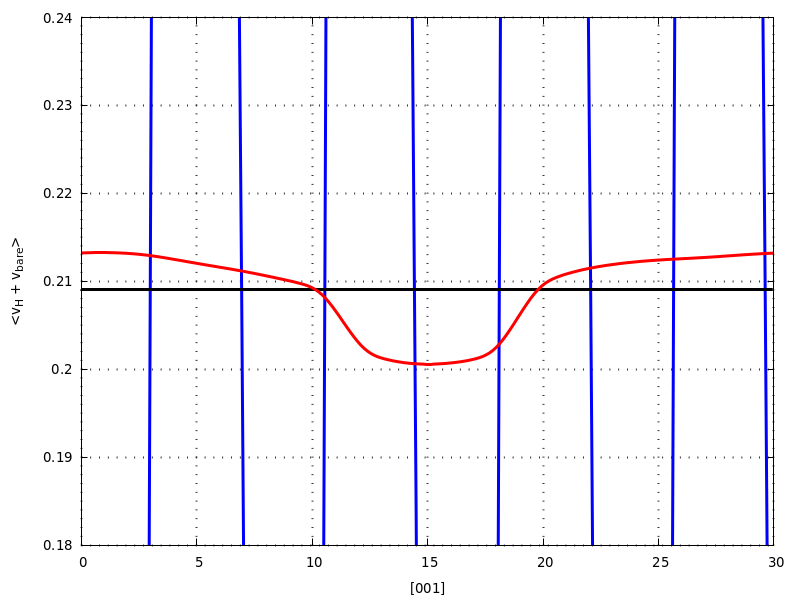
\includegraphics[width=\linewidth]{avg_pot_444_zoom.png}}
%    \end{minipage}
%    \caption[]{}
%    \label{fig:avg-pot}
%\end{figure}

